\pagestyle{plain}
\appendix
\section*{Appendix A: CBOW Vs Skip Gram}
Before the training process is initiated the decision must be made to use a continuous bag of words model or a skip gram model. This decision can have a large effect on the end result of the model produced, it is common practice to train both a CBOW model and a skip gram model as it is difficult to predict which will produce better results in any given use case.
\begin{figure}[H]
\centering
  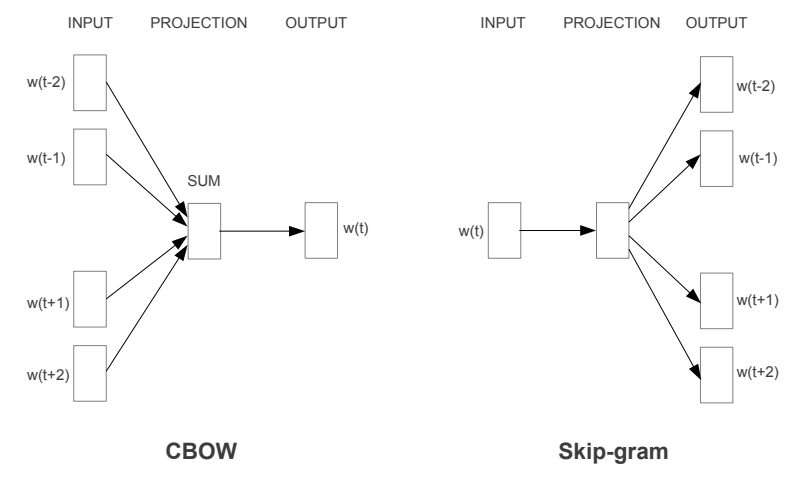
\includegraphics[width=.9\textwidth]{images/CBW_SG.PNG}
  \label{fig:CBOW_SG}
\end{figure}
\noindent
The above figure shows how CBOW predicts the current word based on the context, and the Skip-gram model predicts surrounding words given the current word. While it is said that the skip gram model improves quality of the resulting word vectors by increasing the range of values related to the selected word, this produces an increase in the computational complexity of the process. \cite{Mikolov}


\section*{Appendix B: Parse Tree}
To accurately part of speech tag a piece of text is a computationally complex task, one highly accurate method is to construct a parse tree for the the given corpus. While this is a highly accurate method, the high complexity of the task (higher than polynomial) makes it unpractical for use on a large corpus of text. \cite{Posadas}
\begin{figure}[H]
\centering
  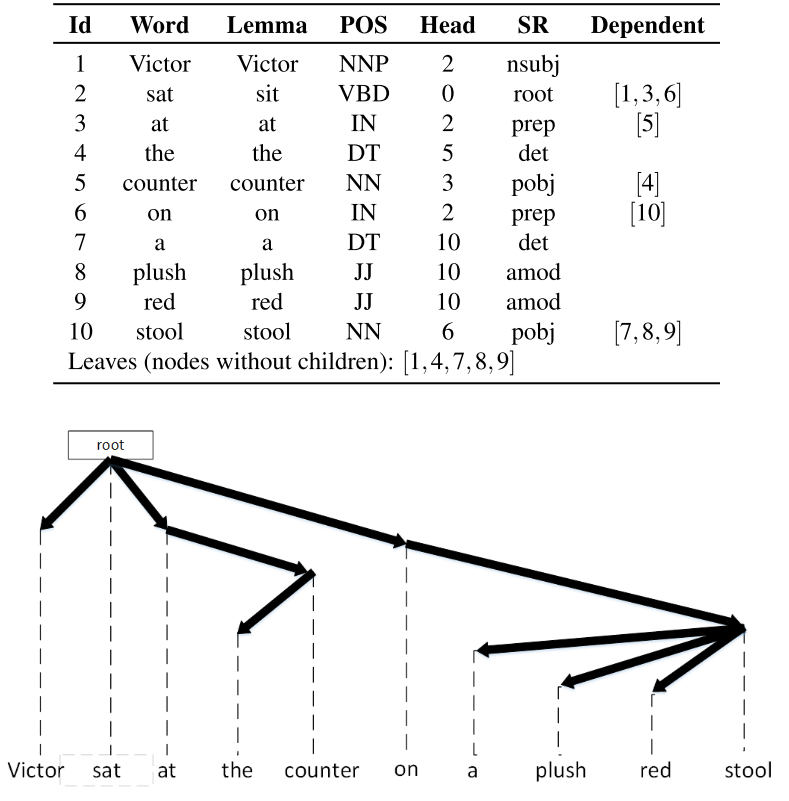
\includegraphics[width=.9\textwidth]{images/parse_tree.PNG}
  \caption{Parse Tree With POS Tags}
  \label{fig:parse_tree}
\end{figure}
\noindent
The above figure \ref{fig:parse_tree} is produced using Stanford CoreNLP and produces the lemmas, POS tags, dependency relations tags and the relations between the elements of the sentence. By structuring the tree in this way a greater understanding of the context of each word is obtained at a cost of computation time. \cite{Qi}

\section*{Appendix C: Training Files}
Download and store a large corpus of Wikipedia text located at: 

\noindent
https://dumps.wikimedia.org/enwiki/ it is recommended to used a corpus which contains at least 1 billion words. Use WikiCorpusExtractor.py to extract can convert xml dump to txt corpus.

\section*{Appendix D: Training Word2Vec}
Use w2v\_train.py passing converted xml dump in txt format as in\_file. Training parameters can be changed here, remove sg=1 to switch to CBOW.

\section*{Appendix E: Training Sense2Vec}
Note Steps 2 and 3 must be preformed on a Linux based system, all others are operating system independent.

\subsection*{Step 1: parse and part of speech (POS) tag each word in the corpus}
Using Training/01\_POS\_Tag.py This process is completed using the stanford parser and uses the following pipelines:

\begin{itemize}
    \item TokenizeProcessor
    \item MWTProcessor
    \item POSProcessor
\end{itemize}
\noindent
No lemmatization is preformed to save processing time with large corpus files, more info found here:
https://stanfordnlp.github.io/stanfordnlp/index.html 
Expects a corpus wile within in\_dir in txt format. Outputs a tagged txt file to the supplied output directory with out\_dir.

\subsection*{Step 2: Build vocabulary and frequency counts}
Using Training/02\_glove\_build\_counts.py, expects a directory of preprocessed .s2v input files and will use GloVe to collect unigram counts and construct and shuffle cooccurrence data. See here for installation instructions: 

\noindent
https://github.com/stanfordnlp/GloVe

\noindent
Using Linix:
Note that this script will call into GloVe and expects you to pass in the
GloVe build directory (/build if you run the Makefile). The commands will
also be printed if you want to run them separately.

\subsection*{Step 3: Train the vectors}
Expects a file containing the shuffled cooccurrences and a vocab file and will output a plain-text vectors file. Note that this script will call into GloVe and expects you to pass in the GloVe build directory (/build if you run the Makefile). The commands will also be printed if you want to run them separately.

\subsection*{Step 4: Export a sense2vec component}
Expects a vectors.txt and a vocab file trained with GloVe and exports a component that can be loaded with Sense2vec.from\_disk.

\section*{Appendix F: Verbs Within Bloom's Taxonomy}
Below is a list of the action verbs used within each level in Bloom's Taxonomy, this data is used within the BloomsTaxonomy.py file to produce section 4.7 in the results chapter. Further details on the used of this hierarchy can be found in Section 2.5.\\
knowledge = ["List", "Name", "Identify", "Reproduce"]\\
understanding = ["Describe", "Explain", "Classify", "Discuss"]\\
application = ["Apply", "Choose", "Employ", "Operate", "Practice"]\\
analysis = ["Compare", "Contrast", "Calculate", "Test", "Analyze"]\\
evaluation = ["Argue", "Assess", "Defend", "Judge", "Summarise"]\\
create = ["Construct", "Compose", "Create", "Design", "Propose"]

\section*{Appendix G: Training Times}
No doubt the most complex step in the training process is part of speech tagging the corpus. With a corpus of 15GB this process took place over four days and required the use of a remote instance in Google Cloud, allowing the use of 28GB of RAM to batch process 50000 words at a time using the Stanford Parser. However once this process was competed training the model using GloVe was faster and produced a more a smaller model than that produced by Word2Vec. Training for Word2Vec using the Gensim library was fast relative to the rest of the process, note this process is much faster once a C compiler is installed. However by taking the POS tagging complexity out of the equation, the training time for Sense2Vec was significantly faster than Word2Vec. The process was completed in approximately a quarter of the time and produced a model a quarter the size compared (980MB) to the Word2Vec model (4.2GB) this process is likely due to the use of the GloVe library. For future work it would be worth investigating the benefits and downsides of using GloVe, Gensim or even FastText to train word embeddings.